\section{Apex Arrow}

The final Repertoire-based action is Apex Arrow (AA), whose usage and damage depends on the level of the Soul Gauge. Regardless of song, the Soul Gauge increments by 5 for each Repertoire proc, up to 100 gauge. The potency of AA increases with gauge and at 80 gauge, using AA allows for the execution of Blast Arrow. AA is generally used on a one minute cadence, though the particular time has flexibility. 

Odd minute AA are used as soon as 100 gauge is reached, or at 21s left on Mage's Ballad and $\ge 80$ gauge is present. If 80 gauge is not present, AA is held until the even minute. Even minute AA usages are only used during burst, even at the expense of holding and over-capping. There is also flexibility with respect to which GCD in the burst window AA is used, so long as AA and Blast Arrow fall under buffs.

These flexible windows also result in the maximum number of Repertoire procs of a particular AA usage being dependent on when exactly the previous AA was used. It is assumed that each AA usage will have $n_{ea} = 4$ Empyreal Arrow usages, although this can be varied by $\pm 1$ depending on the situation. Thus, a minimum of 16 Repertoire procs are required to achieve 100 Soul Gauge. The Soul Gauge distribution is

\begin{equation}
\begin{aligned}
&P_{sg}(k_{sg}; n_r, p_r) = \\
&\begin{cases}
    \displaystyle\sum_{k_r=0}^{15 - n_{ea}} P_r(k_r; n_r, p_r), & k_{sg} = 75 \\ 
    P_r(k_r = k_{sg} / 5 - n_{ea}; n_r, p_r), & 75 < k_{sg} < 100 \\
    \displaystyle\sum_{k_r=20 - n_{ea}}^{n_r} P_r(k_r; n_r, p_r), & k_{sg} = 100
\end{cases}   
\end{aligned}
\end{equation}

Soul Gauge values of $k_{sg} \le 75$ are grouped as a single value (75) as all values represent AA not being used. Soul Gauge values of $k_{sg} \ge 100$ are grouped as a single value (100) due to the gauge cap. If used exactly one minute apart, there are a maximum of $n_r = 20$ Repertoire procs. Soul gauge distributions for various $n_r$ are shown in Figure \ref{fig:aa-sg-distribution}.

\begin{figure}[H]
    \centering
    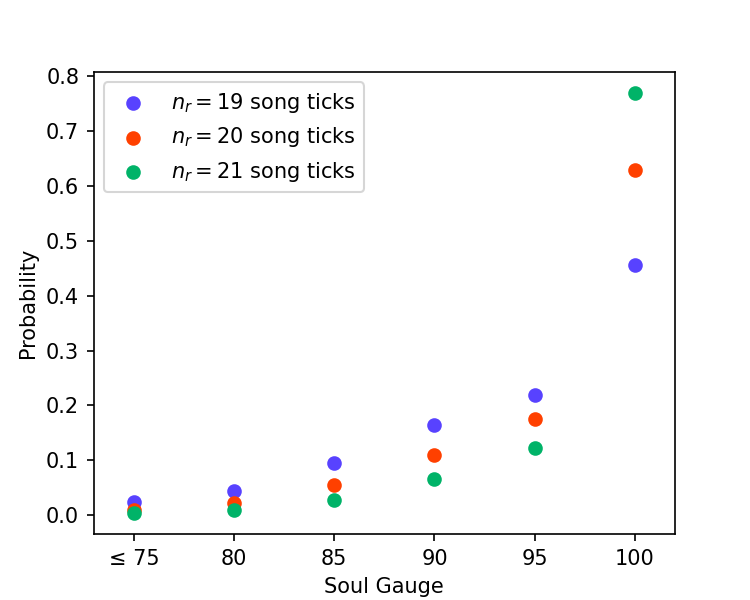
\includegraphics[scale=0.65]{img/aa-sg-distribution.png}
    \caption{Soul Gauge distribution for various maximum Repertoire proc counts.}
    \label{fig:aa-sg-distribution}
\end{figure}

The probability of achieving a full 100 Soul Gauge substantially varies for this range of $n_r$, from 40\% - 80\%.  Additionally, there is a 1\% chance that $\le 75$ Soul Gauge is generated and an AA usage is lost. For modeling damage variability, it is assumed that all AA have $n_r = 20$ to avoid having to track $n_r$ from the previous AA. While some variance is lost, AA is only used once per minute. Additionally, a Soul Gauge difference of 5 results in a potency difference of 30. This potency difference is small enough that it is actually impossible to reliably distinguish the Soul Gauge value of an AA usage in-game based off damage values alone (after accounting for hit type). This occurs because AA damage values with potency differences of up to 30 can overlap due to the game's $\pm 5\%$ damage variance.

Here, the potency of AA is varied instead of the number of usages as given by eqn. \ref{eqn:dmg-mixture}. The damage distribution takes on a slightly different form,

\begin{equation}
    P(D_{aa}) = \sum_{i \in \{75, 80, ..., 100\}} P_{sg}(k_{sg}=i; n_r, p_r)P(D_{aa, i})
\end{equation}

Where $D_i$ is the damage of AA with $i$ Soul Gauge accumulated. As an example, the damage distribution for AA is computed for an even minute AA and odd minute AA. For simplicity, cases where $\le 75$ Soul Gauge is accumulated for both AA usages is omitted. A full list of AA damage values at different Soul Gauge levels is tabulated below

\begin{table}[H]
\centering
\begin{tabular}{@{}ll@{}}
\toprule
Soul Gauge  & Blast Arrow D \\ \midrule
80          & 21,818        \\
85          & 23,181        \\
90          & 24,545        \\
95          & 25,909        \\
100         & 27,272        \\ \bottomrule
\end{tabular}
\end{table}

The AA damage distribution is computed and shown in Figure \ref{fig:aa-dmg-dist}.

\begin{figure}[H]
    \centering
    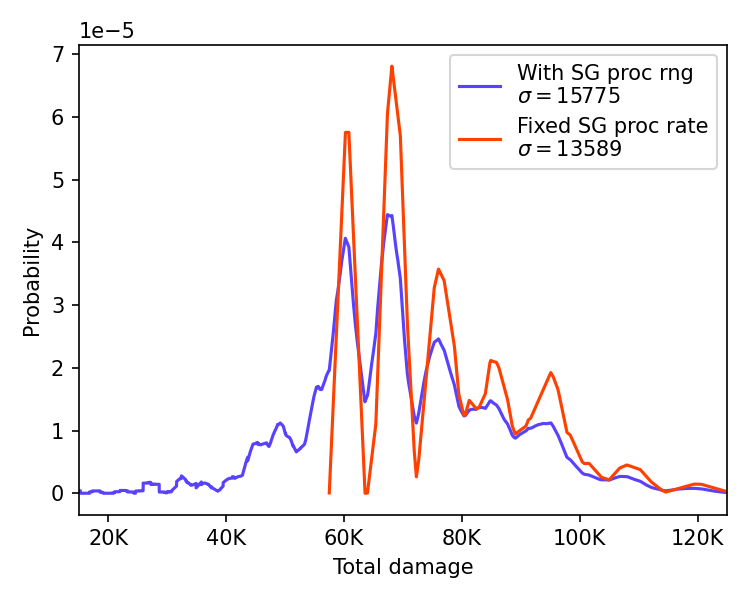
\includegraphics[scale=0.65]{img/aa-dmg-dist.png}
    \caption{Apex Arrow damage distribution for an even minute AA and odd minute AA, for full Soul Gauge variability (blue) and the most probable Soul Gauge values (orange).}
    \label{fig:aa-dmg-dist}
\end{figure}

Accounting for Soul Gauge variability leads to a modest increase in damage variability, with the standard deviation only increasing by 16\%. This intuitively makes sense as the chance of achieving maximum Soul Gauge value is already quite large, where achieving lower values is quite low. The total damage dealt is similar to HS, but with much smaller change in variance. These results suggest that out of all Repertoire-based actions with variability, damage from AA is likely the least variable. In a full rotation, this variability is even further tempered by the guaranteed, 600 potency follow-up attack from Blast Arrow (not included here).